\documentclass[tikz,border=5mm]{standalone}
\begin{document}
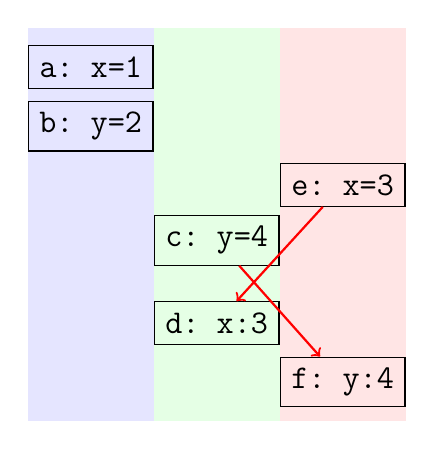
\begin{tikzpicture}

% Background for Column 1
\fill[blue!10] (0.2, 0.5) rectangle (1.8, -4.5);

% Background for Column 2
\fill[green!10] (1.8, 0.5) rectangle (3.4, -4.5);

% Background for Column 3
\fill[red!10] (3.4, 0.5) rectangle (5.0, -4.5);

% Column 1
\node (a) at (1.0, -0.0) [draw, rectangle, inner sep=4pt, font=\large] {\texttt{a:~x=1}};
\node (b) at (1.0, -0.75) [draw, rectangle, inner sep=4pt, font=\large] {\texttt{b:~y=2}};

% Column 2
\node (c) at (2.6, -2.2) [draw, rectangle, inner sep=4pt, font=\large] {\texttt{c:~y=4}};
\node (d) at (2.6, -3.25) [draw, rectangle, inner sep=4pt, font=\large] {\texttt{d:~x:3}};

% Column 3
\node (e) at (4.2, -1.5) [draw, rectangle, inner sep=4pt, font=\large] {\texttt{e:~x=3}};
\node (f) at (4.2, -4.0) [draw, rectangle, inner sep=4pt, font=\large] {\texttt{f:~y:4}};

% Arrows
\draw[->, thick, red] (e) -- (d);
\draw[->, thick, red] (c) -- (f);

\end{tikzpicture}
\end{document}
